\documentclass[11pt,a4paper]{article}
\usepackage[utf8]{inputenc}
\usepackage[english]{babel}
\usepackage{amsmath}
\usepackage{amsfonts}
\usepackage{amssymb}
\usepackage{graphicx}
\usepackage{caption}
\usepackage{subcaption}

\begin{document}

\section{Introduction}
Introduction with example citation \cite{KNUT1984}.

\section{Related work}
\subsection{Preprocessing}
\subsection{Features}
\subsection{Classifying}
\section{Methods and materials}
\subsection{Dataset}
The used dataset consists of two image sets from the \emph{Nationaal Archief}. The first set contains a total of 92 pages and is called Stanford. The second dataset contains 150 pages and is named KNMP. Both sets are divided into even and odd numbered pages. The even pages are used for training and the odd pages are used for evaluating the classifier. One page from both datasets is displayed in figure \ref{fig:dataset}. 

The pages are annotated at word and character level. This means that the coordinates of the words and characters are known as well as their representation. Also the shearing angle of the words known. Not all words of the pages are annotated, only a selection is. In total ... words and ... characters are annotated in the training set and ... words and ... characters in the evaluation set. 
\begin{figure}[hbt]
\centering
\begin{subfigure}[b]{0.4\textwidth}
	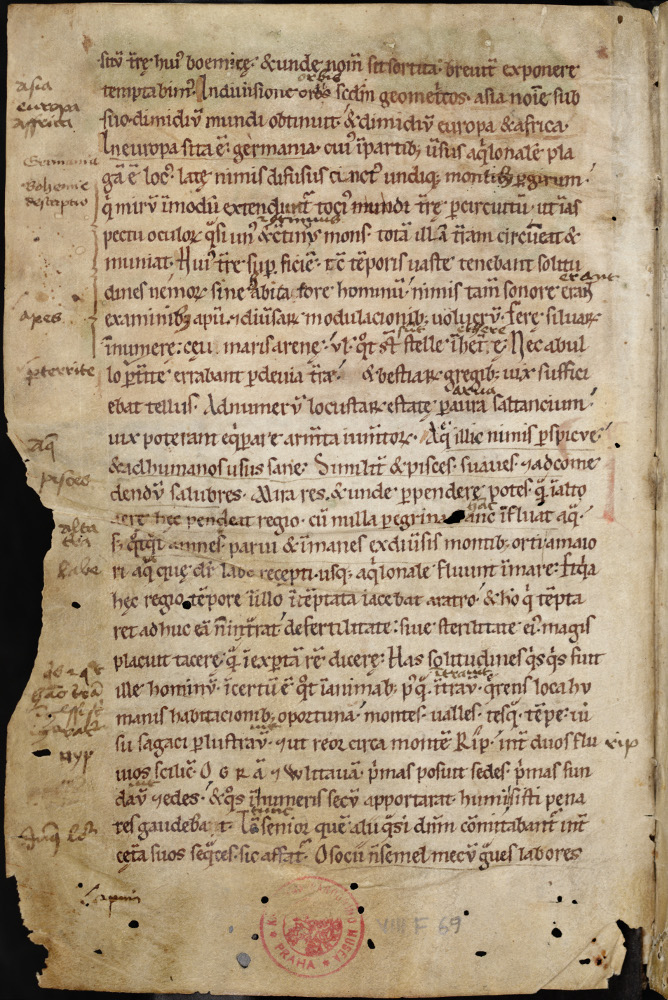
\includegraphics[width=\textwidth]{figures/KNMP4}
	\caption{The 4th page from the KNMP dataset}
\end{subfigure}
\quad
\begin{subfigure}[b]{0.4\textwidth}
	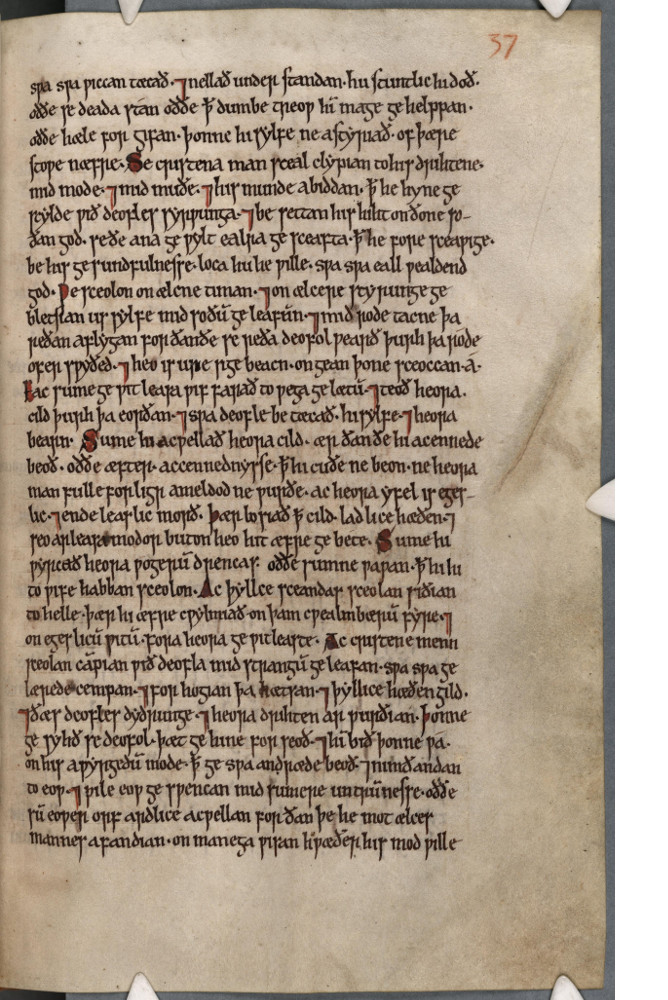
\includegraphics[width=\textwidth]{figures/stanford6}
	\caption{The 6th page from the Stanford dataset}
\end{subfigure}
\caption{Two pages from the two datasets. }
\label{fig:dataset}
\end{figure}


\subsection{Preprocessing}
\subsection{Features}
\subsection{Classifier}
\section{Results}
\section{Discussion}
\bibliographystyle{unsrt}
\bibliography{bibliography}

\end{document}